%!TEX root = ../Thesis.tex
\chapter{Tables}

\section{Estimates and test of the simple linear regression model}
\begin{table}
    \centering
    \begin{tabular}{c:cc|c:cc}
        \hline
        House & Intercept & Temp. & House & Intercept & Temp. \\
        \hline 
        1 & 2.398533 & -0.105537 & 36 & 2.852860 & -0.122672\\
        2 & 3.398808 & -0.137495 & 37 & 6.27161 & -0.36085\\ 
        3 & 4.144182 & -0.203752 & 38 & 3.58106 & -0.20111\\ 
        4 & 2.884192 & -0.186361 & 39 & 6.32565 & -0.38797\\ 
        5 & 3.876744 & -0.192553 & 40 & 4.333811 & -0.223071\\ 
        6 & 2.525637 & -0.111327 & 41 & 3.270357 & -0.209849\\ 
        7 & 2.153872 & -0.119296 & 42 & 2.655654 & -0.112816\\ 
        8 & 6.49637 & -0.28241 & 43 & 3.462811 & -0.180196\\ 
        9 & 1.411321 & -0.077829 & 44 & 1.785110 & -0.082274\\ 
        10 & 16.80251 & -0.76470 & 45 & 25.1895 & -1.1268\\ 
        11 & 2.853030 & -0.121927 & 46 & 2.860330 & -0.153524\\ 
        12 & 4.588960 & -0.210243 & 47 & 1.299755 & -0.088525\\ 
        13 & 4.322333 & -0.171578 & 48 & 3.070152 & -0.162541\\ 
        14 & 5.975906 & -0.292424 & 49 & 3.99257 & -0.18209\\ 
        15 & 3.022654 & -0.160148 & 50 & 4.463920 & -0.195064\\ 
        16 & 4.041873 & -0.224724 & 51 & 4.501192 & -0.204155\\ 
        17 & 8.20034 & -0.40646 & 52 & 4.94798 & -0.33593\\ 
        18 & 1.616462 & -0.068947 & 53 & 2.753387 & -0.152706\\ 
        19 & 4.51546 & -0.19795 & 54 & 3.123352 & -0.166824\\ 
        20 & 1.796715 & -0.111773 & 55 & 2.634592 & -0.110295\\ 
        21 & 2.881053 & -0.123945 & 56 & 2.19092 & -0.09952\\ 
        22 & 2.600607 & -0.154493 & 57 & 3.007890 & -0.128622\\ 
        23 & 4.001741 & -0.180271 & 58 & 2.603941 & -0.115700\\ 
        24 & 4.073325 & -0.183069 & 59 & 3.581131 & -0.181395\\ 
        25 & 7.58839 & -0.30079 & 60 & 4.61306 & -0.25118\\ 
        26 & 5.05844 & -0.22397 & 61 & 3.71516 & -0.17677\\ 
        27 & 2.742857 & -0.121458 & 62 & 3.906559 & -0.173636\\ 
        28 & 30.38456 & -1.64664 & 63 & 11.79446 & -0.50298\\ 
        29 & 4.985258 & -0.231925 & 64 & 2.327872 & -0.122545\\ 
        30 & 4.451597 & -0.227997 & 65 & 2.375351 & -0.128330\\ 
        31 & 4.844060 & -0.253319 & 66 & 5.364626 & -0.264278\\ 
        32 & 2.408233 & -0.082787 & 67 & 3.712356 & -0.145792\\ 
        33 & 3.584799 & -0.158777 & 68 & 4.61927 & -0.22110 \\ 
        34 & 3.778189 & -0.151325 & 69 & 4.022828 & -0.180830 \\ 
        35 & 3.462811 & -0.180196 & 70 & 3.625038 & -0.167733\\
        \hline
    \end{tabular}
    \caption{Estimates of the simple linear regression model}
    \label{tab: est_simple_lm}
\end{table}

\begin{table}
    \centering
    \begin{tabular}{c:cc|c:cc}
        \hline
        House & Shapiro-Wilk & Sign & House & Shapiro-Wilk & Sign \\
        \hline 
        1 & 7.458816e-09 & 0.154571 & 36 & 0.6551522 & 0.604916 \\
        2 & 0.03683475 & 0.897101 & 37 & 0.00211908&0.437686 \\ 
        3 & 0.1522292 & 0.897101 & 38 & 0.09384231&0.244235 \\ 
        4 & 0.1385351 & 0.897101 & 39 & 0.720376& 0.853408 \\ 
        5 & 0.4889633 & 0.897101 & 40 & 0.0814062 &0.698022\\ 
        6 & 0.06605537 & 0.579290 & 41 & 0.7499187 & 0.698022\\ 
        7 & 1.77266e-08 & 0.000096 & 42 & 0.5544048 & 0.195667\\ 
        8 & 0.001297956 & 0.579290 & 43 & 0.9688807 & 0.853408\\ 
        9 & 0.002104755 & 0.355280 & 44 & 0.05668529 & 0.795902\\ 
        10 & 0.130679 & 0.704379 & 45 & 0.678235& 0.517817\\ 
        11 & 0.709406 & 0.698022 & 46 & 0.2546043 & 1\\ 
        12 & .319923e-07 & 0.437686 & 47 & 0.001065575 & 0.002847\\ 
        13 & 0.0001239323 & 0.853408 & 48 & 4.674662e-09 & 0.897101\\
        14 & 0.2859703 & 0.517817 & 49 & 0.0352531 & 0.698022\\ 
        15 & 0.877681 & 1 & 50 & 0.9042102 &0.604916\\ 
        16 & 0.03106733 & 1 & 51 & 0.2314035 & 0.459691\\ 
        17 & 0.4268815 & 0.579290 & 52 & 0.02903943 & 0.795902\\ 
        18 & 1.30237e-05 & 0.300679 & 53 & 0.4957589 & 1\\ 
        19 & 0.809942 & 0.355280 & 54 & 0.04954421 & 0.195667\\ 
        20 & 0.3582973& 0.711703 & 55 & 0.2428003 & 0.437686\\ 
        21 & 0.1858593& 0.517817 & 56 & 0.09574403 & 1\\ 
        22 & 0.07530409 & 1 & 57 & 0.0213735 & 0.795902\\ 
        23 & 0.006563705 & 0.300679 & 58 & 0.7065081 & 0.897101\\ 
        24 & 0.9487515& 0.579290 & 59 & 0.07945885 & 0.711703 \\ 
        25 & 0.2231339 & 0.459691 & 60 &  0.5896005 & 1\\ 
        26 & 0.002878431& 0.355280 & 61 & 5.313489e-06 & 0.019687\\
        27 & 0.5797924 & 1 & 62 & 0.001550156 & 0.355280\\ 
        28 & 0.008843725& 0.300679 & 63 & 0.5771746 & 0.853408\\ 
        29 & 0.006802018&0.365187 & 64 & 0.006368894 & 0.517817\\ 
        30 & 0.08408281&0.897101 & 65 & 0.01968257 & 0.195667\\ 
        31 & 0.001679153& 1 & 66 & 0.0006757623 & 0.604916\\ 
        32 & 8.699853e-07& 0.013802 & 67 & 0.1761617 & 1\\ 
        33 & 0.917481&0.517817 & 68 & 0.2359113 & 0.579290\\ 
        34 & 4.238303e-05&0.517817 & 69 & 0.008934653 &0.579290 \\ 
        35 & 0.9688807&0.853408 & 70 & 0.8963474 & 0.267182\\
        \hline
    \end{tabular}
    \caption{P-values from Shapiro-Wilk test and sign test on the simple linear regression model}
    \label{tab: shapiro_simple_lm}
\end{table}

\section{Estimates and test of the multiple linear regression model}
\subsection{Significance of parameters for full model}
\begin{table}
    \centering
    \resizebox{!}{0.48\textwidth}{\begin{tabular}{ccccccccccccccccccccc}
     \hline
     Index & I & T & N & E & S & W & MSL & SR & WB & SB & AB & CB & WKND & T:N & T:E & T:S & T:W \\
    \hline
     1 &  & \Minus*** &  & \Plus. &  & \Plus*** & \Plus* & & & \Minus*** & \Minus*** &  &  &  &  & \Plus. & \Minus*** & \\
     2 & \Plus** &\Minus*** & &\Plus** & &\Plus*** & &\Minus* & &\Minus* & &\Plus* & & & &  &\Minus*** \\
     3 &  &\Minus*** & &\Plus*** & &\Plus*** &\Plus*** &\Minus*** &\Plus. & &\Minus* & & & & &\Plus** &\Minus* \\
     4 & \Minus* &\Minus*** &\Plus* & &\Plus*** & &\Plus** &\Minus*** & & & & & & & & & \\
     5 & &\Minus*** & &\Plus*** & &\Plus*** &\Plus*** &\Minus*** &\Plus** &\Plus*** & & & &\Plus* & &\Plus*** &\Minus** \\
     7 &\Plus*** &\Minus*** &\Minus** &\Plus*** &\Minus** &\Plus** &\Minus*** &\Plus** & \Plus* &\Plus*** & & & & &\Minus*** &\Plus* &\Minus** \\
     11 &\Plus** &\Minus*** & &\Plus*** & &\Plus*** & &\Minus*** &\Plus*** & & &\Plus* & & & &\Plus** & \\
     12 &  &\Minus*** & & & &\Plus* & & & & & & &\Minus* & & & & \\
     14 &\Plus* &\Minus*** & &\Plus*** & &\Plus*** & &\Minus** &\Plus*** & &\Minus* & & & & &\Plus** & \\
     18 &\Plus*** &\Minus* & &\Plus*** &\Minus* &\Plus** &\Minus** &\Plus. & & &\Minus. & & & & &\Plus** &\Minus*** \\
     21 &\Plus** &\Minus*** & &\Plus* & & \Plus*** & &  & &\Plus* & & & &  &  &  & \Minus***\\
     22 & &\Minus*** & & &\Plus*** &\Plus** & &\Minus*** & &\Minus** & &\Plus. & &  & & \Minus* \\
     23 &\Plus* &\Minus*** &\Minus. &\Plus* & &\Plus*** & &\Minus*** & & &\Minus. & & & & &\Plus*** &\Minus*** \\
     28 & &\Minus*** & &\Plus** & &\Plus. & &\Minus*** & &\Minus* & &\Minus*** &\Minus*** & & & & \\
     29 &\Plus. &\Minus*** & &\Plus*** & &\Plus*** & &\Minus** &\Minus* &\Plus. & & & &\Plus. & &\Plus* &\Minus*** \\
     30 &\Plus. &\Minus*** & &\Plus*** & &\Plus*** & &\Minus*** &\Plus* &\Minus* & & & & & &\Plus. &\Minus.\\
     31 & &\Minus*** & &\Plus*** & &\Plus*** &\Plus** &\Minus*** &\Plus. & &\Minus. & & &\Plus** & &\Plus*** &\Minus*** \\
     32 & &\Minus** & & &\Plus* &\Plus*** & & &\Minus** &\Minus* & & & & &\Plus* & &\Minus* \\
     33 & &\Minus*** & &\Plus*** & & & &\Minus** \\
     34 &\Plus. &\Minus*** & &\Plus*** &\Plus. &\Plus*** & &\Minus** & & &\Minus* &\Plus*** &\Minus* & & & & *\\
     36 &\Plus** &\Minus*** & &\Plus*** & &\Plus** & &\Minus*** & & & & &\Minus* & & &\Plus** & \\
     37 & &\Minus*** & &\Plus*** &\Plus** &\Plus** & &\Minus*** & & & & & & & & & \\
     38 &\Minus*** &\Minus*** & &\Plus** & &\Plus*** &\Plus*** &\Minus*** &\Plus** &\Minus. & & &\Minus* &\Plus. & &\Plus. &\Minus*** \\
     40 &\Plus* &\Minus*** & &\Plus* &\Plus** &\Plus** & &\Minus*** & &\Minus** &\Minus* & & & & &\Plus. &\Minus* \\
     41 & \Plus*** &\Minus*** & &\Plus*** & &\Plus*** &\Minus. & &\Plus. & &\Minus. & & & & &\Plus. &\Minus.\\
     42 & &\Minus*** & &\Plus*** & &\Plus*** &\Plus*** &\Minus*** &\Plus. & & & &\Minus*** & & &\Plus* &\Minus* \\
     44 & &\Minus*** &\Minus* & & & & &\Minus** & & & &\Plus** & & & &\Plus** & \\
     45 &\Plus** & \Minus*** & & &\Plus* &\Plus*** & &\Minus. & & & &\Plus* & & &\Plus* &\Plus. &\Minus** \\
     46 & &\Minus*** & &\Plus* &\Plus* &\Plus** & &\Minus** & & & & &\Minus* & & & &\Minus** \\
     47 & &\Minus*** & &\Plus** &\Plus* &\Plus*** &\Plus. &\Minus* &\Minus. & & &\Plus*** &\Plus*** & &\Minus** & &\Minus*** \\
     48 &\Plus* &\Minus*** & &\Plus** & &\Plus** & &\Minus** &\Plus** & & & &\Minus*** & & & &\Minus** \\
     49 &\Plus* &\Minus*** & & & & & &\Minus** & &\Plus* & & & & & & & \\
     50 & &\Minus*** &\Minus* &\Plus*** &\Minus** &\Plus* & &\Minus*** &\Plus** & & & & &\Plus. & &\Plus*** & \\
     52 &\Plus. &\Minus*** &\Minus* &\Plus* &\Minus* & & &\Minus** &\Minus*** &\Minus*** & &\Minus*** & &\Plus. & &\Plus*** & \\
     54 & &\Minus*** & &\Plus** & &\Plus** & &\Minus*** & & & &\Minus. &\Minus* & & &\Plus** &\Minus* \\
     55 & &\Minus*** & &\Plus* & &\Plus*** &\Plus* &\Minus*** & & & &\Minus. &\Minus* & & &\Plus*** &\Minus* \\
     56 &\Plus** &\Minus*** & &\Plus** & &\Plus*** & &\Minus** &\Minus. & &\Minus* & & & & &\Plus* &\Minus* \\
     57 &\Plus. &\Minus*** & &\Plus*** & &\Plus** & & & & & & & & & & &\Minus* \\
     58 & &\Minus*** &\Minus. &\Plus. & &\Plus*** & &\Minus*** & & & &\Plus** & &\Plus* & &\Plus*** &\Minus* \\
     61 &\Plus*** &\Minus*** & &\Plus** & &\Plus** &\Minus*** &\Plus. &\Plus** & & &\Minus. & &\Minus. & & & \\
     64 & &\Minus*** &\Minus* &\Plus*** & &\Plus** & &\Minus*** &\Plus. & & & &\Minus* & &\Minus* &\Plus** &\Minus** \\
     65 & &\Minus*** & &\Plus* & &\Plus*** & &\Minus*** & & & & & & & &\Plus* &\Minus** \\
     66 & &\Minus*** & &\Plus*** &\Plus* &\Plus*** & &\Minus*** & &\Minus. &\Minus. & & & & &\Plus** &\Minus** \\
    \hline
    \end{tabular}}
    \caption{Significance of parameters from the full multiple linear regression model performed on 'long' houses}
    \label{tab: lmMult_full_L}
\end{table}

\begin{table}
    \centering
    \resizebox{!}{0.33\textwidth}{\begin{tabular}{ccccccccccccccccccc}
     \hline
     Index & I & T & N & E & S & W & MSL & SR & AB & CB & WKND & T:N & T:E & T:S & T:W \\
    \hline
    6&   & \Minus *** &   & \Plus * &   & \Plus ** &   & \Minus * & \Minus .  &   &   &   &   &   & \\
8& \Plus ** & \Minus *** &   & \Plus * &   & \Plus *** &   & \Minus * &   &   &   &   &   & \Plus . & \Minus *\\
9&   & \Minus *** & \Minus .  &   &   & \Plus ** & \Plus ** & \Minus *** & \Minus * &   & \Minus * & \Plus . &   & \Plus * & \Minus ** \\
10&   & \Minus *** &   & \Plus *** &   & \Plus *** & \Plus . & \Minus ** &   &   & \Minus ** & \Plus . &   &   & \Minus * \\
13&   & \Minus *** &   & \Plus * &   & \Plus ** & \Plus * & \Minus * &   &   & \Minus .  & \Plus . &   & \Plus ** & \Minus *\\
15&   & \Minus *** &   & \Plus *** &   & \Plus ** &   & \Minus .  &   & \Minus .  & \Minus .  &   &   &   & \Minus . \\
16&   & \Minus *** &   & \Plus * &   & \Plus *** & \Plus . & \Minus * &   &   &   &   &   &   & \Minus ** \\
17&   & \Minus *** &   & \Plus ** & \Plus ** & \Plus *** &   & \Minus ** &   &   & \Minus .  &   &   &   & \Minus *** \\
19&   & \Minus *** &   & \Plus ** & \Minus .  &   & \Plus . & \Minus .  &   &   & \Minus .  & \Plus . &   & \Plus ** & \\
20&   & \Minus *** &   &   & \Plus * &   &   &   &   &   &   &   &   &   & \\
24&   & \Minus *** &   & \Plus * &   & \Plus *** & \Plus * &   &   &   &   &   &   &   & \Minus *** \\ 
25&   & \Minus *** &   & \Plus ** &   & \Plus *** &   &   & \Minus .  &   &   &   &   & \Plus . & \Minus * \\
26&   & \Minus *** &   & \Plus . & \Plus . & \Plus *** & \Plus * & \Minus ** & \Minus *** &   &   &   &   &   & \Minus * \\
27&   & \Minus *** &   & \Plus * & \Plus ** & \Plus *** &   &   &   & \Minus * &   &   &   &   & \Minus * \\
35&   & \Minus *** &   & \Plus ** & \Plus * & \Plus *** &   & \Minus ** &   & \Plus * &   &   &   &   & \Minus ** \\
39& \Plus ** & \Minus *** &   &   &   & \Plus * & \Minus * & \Minus .  &   &   & \Minus .  &   &   &   & \\
43&   & \Minus *** &   & \Plus ** & \Plus * & \Plus *** &   & \Minus ** &   & \Plus * &   &   &   &   & \Minus ** \\
51&   & \Minus *** &   & \Plus . &   & \Plus *** &   & \Minus ** &   &   & \Minus * &   &   & \Plus * & \Minus * \\
53&   & \Minus *** &   & \Plus * &   & \Plus * &   &   &   &   &   &   &   &   & \Minus . \\
59&   & \Minus *** & \Minus .  & \Plus *** & \Plus * & \Plus *** &   & \Minus .  &   &   &   & \Plus . &   & \Plus . & \Minus . \\
60&   & \Minus *** & \Minus * & \Plus ** & \Plus . & \Plus *** &   & \Minus *** &   &   &   & \Plus * &   & \Plus * & \Minus *** \\
62& \Plus * & \Minus *** &   &   &   & \Plus * &   & \Minus .  & \Minus * &   &   &   &   &   & \\
63& \Plus . & \Minus *** &   & \Plus * &   &   &   &   &   &   & \Minus ** &   &   & \Plus . & \\
67& \Plus * & \Minus *** &   & \Plus *** &   & \Plus *** &   & \Minus *** & \Plus . & \Plus * &   &   & \Minus * & \Plus . & \Minus ** \\
68&   & \Minus *** &   &   &   & \Plus * &   & \Minus *** &   & \Plus * & \Minus ** &   &   & \Plus * & \Minus * \\
69&   & \Minus *** &   &   & \Plus . & \Plus ** &   & \Minus .  & \Minus *** &   &   &   & \Plus . &   & \\
70&   & \Minus *** &   & \Plus . & \Plus . & \Plus *** & \Plus ** & \Minus *** &   &   &   &   &   &   & \Minus * \\

    \hline
    \end{tabular}}
    \caption{Significance of parameters from the full multiple linear regression model performed on 'short' houses}
    \label{tab: lmMult_full_S}
\end{table}

\section{Tests of residuals from multiple linear regression model}
\begin{table}
    \centering
    \begin{tabular}{c:cc|c:cc}
        \hline
        House & P-value & Sign & House & P-value & Sign \\
        \hline 
        1 & 1.269662e-07 & 0.604916 & 36 & 0.0318435 & 0.897101\\
        2 & 0.2120532 & 0.365187 &  37 & 0.5588932 & 0.897101\\ 
        3 & 0.06289541 & 0.897101 & 38 & 0.002469713 & 0.244235\\ 
        4 & 0.1693807 & 0.897101 & 39 & 0.1319804 & 0.579290\\ 
        5 & 0.9020079 & 1 & 40 & 0.2151643 & 1\\ 
        6 & 0.511858 & 1 & 41 & 0.7165372 & 0.604916\\ 
        7 & 2.400099e-10 & 0.006472 & 42 & 0.5484956 & 1\\ 
        8 & 0.3662207 & 0.355280 & 43 & 0.8539095 & 0.853408\\ 
        9 & 0.01292524 & 0.195349 & 44 & 0. 09057111 & 0.517817\\ 
        10 & 0.5039661 & 0.254605 & 45 & 0.8307638 & 0.897101\\ 
        11 & 0.2445798 & 1 & 46 & 0.7925841 & 1\\ 
        12 & 5.838099e-06 & 0.092399 & 47 & 1.763434e-05 & 0.120377\\
        13 & 0.01173622 & 0.853408 & 48 & 4.364622e-05 & 0.517817\\
        14 & 0.2712269 & 0.517817 & 49 & 0.09749062 & 0.517817\\ 
        15 & 0.9682545 & 0.853408 & 50 & 0.6649854 & 0.897101\\ 
        16 & 0.07409811& 1 & 51 & 0.6341959 & 1\\ 
        17 & 0.9973268& 1 & 52 & 4.159959e-05 & 0.437686\\ 
        18 & 1.017533e-06 & 0.365187 & 53 & 0.4897047 & 0.853408\\ 
        19 & 0.2113022 & 1 & 54 & 0.008756327 & 0.154571\\ 
        20 & 0.6677595 & 0.711703 & 55 & 0.5201494 & 0.517817\\ 
        21 & 0.155591 & 0.897101 & 56 & 0.4827258 & 0.795902\\ 
        22 & 0.003089513 & 1 & 57 & 0.005584645 & 0.795902\\ 
        23 & 0.09877236 & 0.698022 & 58 & 0.4809962 & 0.698022\\ 
        24 & 0.461353 & 0.853408 & 59 & 0.6763879 & 1\\ 
        25 & 0.9855876 & 0.459691 & 60 & 0.6583508 & 0.711703\\ 
        26 & 0.01226589 & 0.459691 & 61 & 2.841694e-05 & 0.052087\\
        27 & 0.5094042 & 0.853408 & 62 & 0.009033716 & 0.267182\\ 
        28 & 0.5752663 & 0.019687 & 63 & 0.6070834 & 0.355280\\ 
        29 & 0.1056845 & 0.698022 & 64 & 0.002157001 & 0.795902\\ 
        30 & 0.4512082 & 0.517817 & 65 & 0.09290001 & 0.437686\\ 
        31 & 0.4481276 & 0.300679 & 66 & 0.002398244 & 0.795902\\ 
        32 & 4.134475e-08 & 0.038238 & 67 & 0.735418 & 1\\ 
        33 & 0.4464175 & 0.795902 & 68 & 0.2093689 & 0.853408\\ 
        34 & 5.011367e-06 & 0.604916 & 69 & 0.0001833683 & 0.195349\\
        35 & 0.8539095 & 0.853408 & 70 & 0.1393319 & 1 \\
        \hline
    \end{tabular}
    \caption{P-values from Shapiro-Wilk test for normality on the general multiple linear regression model}
    \label{tab: shapiro_multiple_lm}
\end{table}

\subsection{Significance of parameters for general regression model}
\begin{table}
    \centering
    \begin{tabular}{cccccccccccc}
     \hline
     Index & I & T & N & E & S & W & SR & T:N & T:E & T:S & T:W \\
    \hline
    1& \Plus *** & \Minus *** &  &  &  & \Plus ** &  &  &  & \Plus . & \Minus ** \\
2& \Plus *** & \Minus *** &  & \Plus ** &  & \Plus *** & \Minus *** &  &  &  & \Minus *** \\
3& \Plus *** & \Minus *** &  & \Plus *** &  & \Plus *** & \Minus *** &  &  & \Plus * & \Minus * \\
4& \Plus *** & \Minus *** & \Plus * &  & \Plus *** &  & \Minus *** &  &  &  &  \\
5& \Plus *** & \Minus *** &  & \Plus *** &  & \Plus *** & \Minus *** & \Plus * &  & \Plus *** & \Minus ** \\
7& \Plus *** & \Minus *** & \Minus ** & \Plus *** & \Minus . & \Plus ** & \Plus *** &  & \Minus ** & \Plus * & \Minus ** \\
11& \Plus *** & \Minus *** &  & \Plus *** &  & \Plus *** & \Minus *** &  &  & \Plus * &  \\
12& \Plus *** & \Minus *** &  & \Plus . &  & \Plus * &  &  &  &  &  \\
14& \Plus *** & \Minus *** &  & \Plus *** &  & \Plus *** & \Minus ** &  &  & \Plus ** &  \\
18& \Plus *** & \Minus ** &  & \Plus *** & \Minus ** & \Plus ** & \Plus . &  &  & \Plus *** & \Minus *** \\
21& \Plus *** & \Minus *** &  & \Plus * &  & \Plus *** &  &  &  &  & \Minus *** \\
22& \Plus *** & \Minus *** &  &  & \Plus *** & \Plus ** & \Minus *** &  &  &  & \Minus * \\
23& \Plus *** & \Minus *** & \Minus . & \Plus * &  & \Plus *** & \Minus *** &  &  & \Plus *** & \Minus *** \\
28& \Plus *** & \Minus *** &  & \Plus * & \Plus . &  & \Minus ** &  &  &  &  \\
29& \Plus *** & \Minus *** &  & \Plus *** &  & \Plus *** & \Minus ** & \Plus * &  & \Plus ** & \Minus *** \\
30& \Plus *** & \Minus *** &  & \Plus * & \Plus . & \Plus *** & \Minus *** &  &  &  & \Minus * \\
31& \Plus *** & \Minus *** &  & \Plus *** &  & \Plus *** & \Minus *** & \Plus ** &  & \Plus *** & \Minus *** \\
32& \Plus *** & \Minus ** &  &  & \Plus . & \Plus ** &  &  & \Plus . &  & \Minus . \\
33& \Plus *** & \Minus *** &  & \Plus *** & \Plus ** & \Plus *** & \Minus *** &  &  &  & \Minus ** \\
34& \Plus *** & \Minus *** &  & \Plus *** & \Plus . & \Plus *** & \Minus ** &  &  & \Plus . & \Minus ** \\
36& \Plus *** & \Minus *** &  & \Plus *** &  & \Plus *** & \Minus *** &  &  & \Plus ** &  \\
37& \Plus *** & \Minus *** &  & \Plus *** & \Plus ** & \Plus ** & \Minus *** &  &  &  &  \\
38& \Plus *** & \Minus *** &  & \Plus * &  & \Plus *** & \Minus *** &  &  &  & \Minus *** \\
40& \Plus *** & \Minus *** &  & \Plus . & \Plus ** & \Plus ** & \Minus *** &  & \Plus . & \Plus * & \Minus * \\
41& \Plus *** & \Minus *** &  & \Plus *** & \Plus . & \Plus *** &  &  & \Plus . & \Plus . & \Minus . \\
42& \Plus *** & \Minus *** &  & \Plus *** &  & \Plus *** & \Minus *** &  &  &  & \Minus * \\
44& \Plus *** & \Minus *** & \Minus * &  &  &  & \Minus ** &  &  & \Plus * &  \\
45& \Plus *** & \Minus *** &  &  & \Plus * & \Plus *** & \Minus * &  & \Plus * & \Plus * & \Minus *** \\
46& \Plus *** & \Minus *** &  & \Plus * & \Plus * & \Plus *** & \Minus ** &  &  &  & \Minus ** \\
47& \Plus *** & \Minus *** &  & \Plus ** &  & \Plus *** & \Minus ** &  & \Minus ** &  & \Minus *** \\
48& \Plus *** & \Minus *** &  & \Plus ** & \Plus * & \Plus *** & \Minus ** &  &  &  & \Minus ** \\
49& \Plus *** & \Minus *** &  &  &  &  & \Minus ** &  &  &  &  \\
50& \Plus *** & \Minus *** & \Minus . & \Plus *** & \Minus * & \Plus ** & \Minus *** & \Plus . &  & \Plus *** & \Minus . \\
52& \Plus *** & \Minus *** & \Minus . &  & \Minus ** & \Minus . & \Minus *** &  &  & \Plus *** &  \\
54& \Plus *** & \Minus *** &  & \Plus ** &  & \Plus ** & \Minus *** &  &  & \Plus * & \Minus * \\
55& \Plus *** & \Minus *** &  & \Plus * & \Plus . & \Plus *** & \Minus *** &  &  & \Plus ** & \Minus * \\
56& \Plus *** & \Minus *** &  & \Plus ** &  & \Plus *** & \Minus *** &  &  & \Plus ** & \Minus * \\
57& \Plus *** & \Minus *** &  & \Plus *** &  & \Plus *** &  &  &  &  & \Minus ** \\
58& \Plus *** & \Minus *** & \Minus . & \Plus . &  & \Plus *** & \Minus *** & \Plus * &  & \Plus *** & \Minus ** \\
61& \Plus *** & \Minus *** &  & \Plus * & \Plus . & \Plus * &  & \Minus . &  & \Minus . &  \\
64& \Plus *** & \Minus *** & \Minus * & \Plus *** &  & \Plus *** & \Minus *** &  & \Minus . & \Plus ** & \Minus ** \\
65& \Plus *** & \Minus *** &  & \Plus * &  & \Plus *** & \Minus *** &  &  & \Plus * & \Minus ** \\
66& \Plus *** & \Minus *** & \Plus . & \Plus *** & \Plus ** & \Plus *** & \Minus *** &  &  & \Plus ** & \Minus ** \\
    \hline
    \end{tabular}
    \caption{Significance of parameters for 'long' houses}
    \label{tab: lmMult_gen_L}
\end{table}
\begin{table}[H]
    \centering
    \begin{tabular}{cccccccccccc}
     \hline
     Index & I & T & N & E & S & W & SR & T:N & T:E & T:S & T:W \\
    \hline
6& \Plus *** & \Minus *** &  & \Plus . &  & \Plus ** & \Minus * &  &  &  &  \\
8& \Plus *** & \Minus *** &  & \Plus * &  & \Plus *** & \Minus * &  &  & \Plus * & \Minus . \\
9& \Plus *** & \Minus *** & \Minus . &  &  & \Plus * & \Minus *** & \Plus * &  & \Plus * & \Minus ** \\
10& \Plus *** & \Minus *** &  & \Plus *** &  & \Plus ** & \Minus ** &  &  &  & \Minus . \\
13& \Plus *** & \Minus *** &  & \Plus . &  & \Plus ** & \Minus . & \Plus . &  & \Plus ** & \Minus ** \\
15& \Plus *** & \Minus *** &  & \Plus ** &  & \Plus ** &  &  &  &  &  \\
16& \Plus *** & \Minus *** &  & \Plus . &  & \Plus *** & \Minus * &  &  &  & \Minus ** \\
17& \Plus *** & \Minus *** &  & \Plus * & \Plus *** & \Plus *** & \Minus ** &  &  &  & \Minus *** \\
19& \Plus *** & \Minus *** &  & \Plus * & \Minus . &  &  & \Plus . &  & \Plus ** &  \\
20& \Plus *** & \Minus *** &  &  & \Plus * &  &  &  &  &  &  \\
24& \Plus *** & \Minus *** &  & \Plus * &  & \Plus *** &  &  &  &  & \Minus *** \\
25& \Plus *** & \Minus *** &  & \Plus ** &  & \Plus *** &  &  &  & \Plus * & \Minus * \\
26& \Plus *** & \Minus *** &  &  &  & \Plus *** & \Minus * & \Plus . &  & \Plus * & \Minus * \\
27& \Plus *** & \Minus *** &  & \Plus . & \Plus ** & \Plus ** &  &  &  &  & \Minus * \\
35& \Plus *** & \Minus *** &  & \Plus ** & \Plus . & \Plus *** & \Minus ** &  &  &  & \Minus ** \\
39& \Plus *** & \Minus *** &  &  &  & \Plus * & \Minus * &  &  & \Plus . &  \\
43& \Plus *** & \Minus *** &  & \Plus ** & \Plus . & \Plus *** & \Minus ** &  &  &  & \Minus ** \\
51& \Plus *** & \Minus *** &  &  & \Plus . & \Plus *** & \Minus ** &  &  & \Plus * & \Minus ** \\
53& \Plus *** & \Minus *** &  & \Plus * &  & \Plus * &  &  &  &  & \Minus . \\
59& \Plus *** & \Minus *** & \Minus * & \Plus ** & \Plus * & \Plus *** & \Minus * & \Plus * &  & \Plus * & \Minus . \\
60& \Plus *** & \Minus *** & \Minus * & \Plus ** &  & \Plus *** & \Minus *** & \Plus ** &  & \Plus ** & \Minus *** \\
62& \Plus *** & \Minus *** &  &  &  & \Plus * & \Minus * &  &  &  &  \\
63& \Plus *** & \Minus *** &  & \Plus * &  &  &  &  &  & \Plus . &  \\
67& \Plus *** & \Minus *** &  & \Plus *** &  & \Plus *** & \Minus *** &  & \Minus * & \Plus . & \Minus ** \\
68& \Plus *** & \Minus *** &  &  &  & \Plus * & \Minus *** &  &  & \Plus * & \Minus * \\
69& \Plus *** & \Minus *** &  &  &  & \Plus ** & \Minus * &  & \Plus * &  &  \\
70& \Plus *** & \Minus *** &  & \Plus . &  & \Plus *** & \Minus *** &  &  &  & \Minus ** \\
    \hline
    \end{tabular}
    \caption{Significance of parameters for 'short' houses}
    \label{tab: lmMult_gen_S}
\end{table}


\chapter{Figures}
\begin{figure}
    \centering
    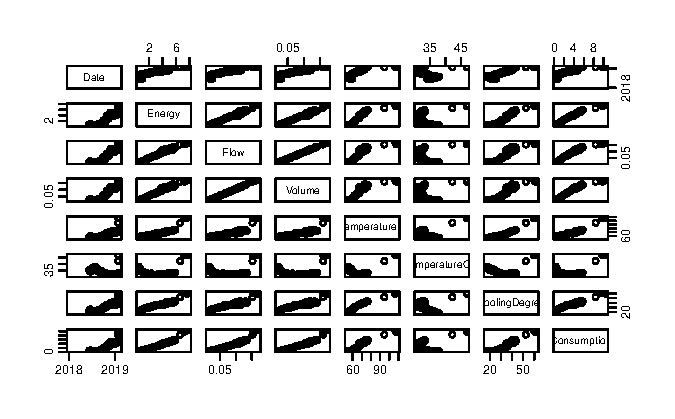
\includegraphics[width=1.3\textwidth, angle = 90 ]{../../../figures/house_attri.pdf}
    \caption{Scatterplot showing the average of relevant attributes from house data}
    \label{fig: house_attri}
\end{figure}

\begin{figure}
    \centering
    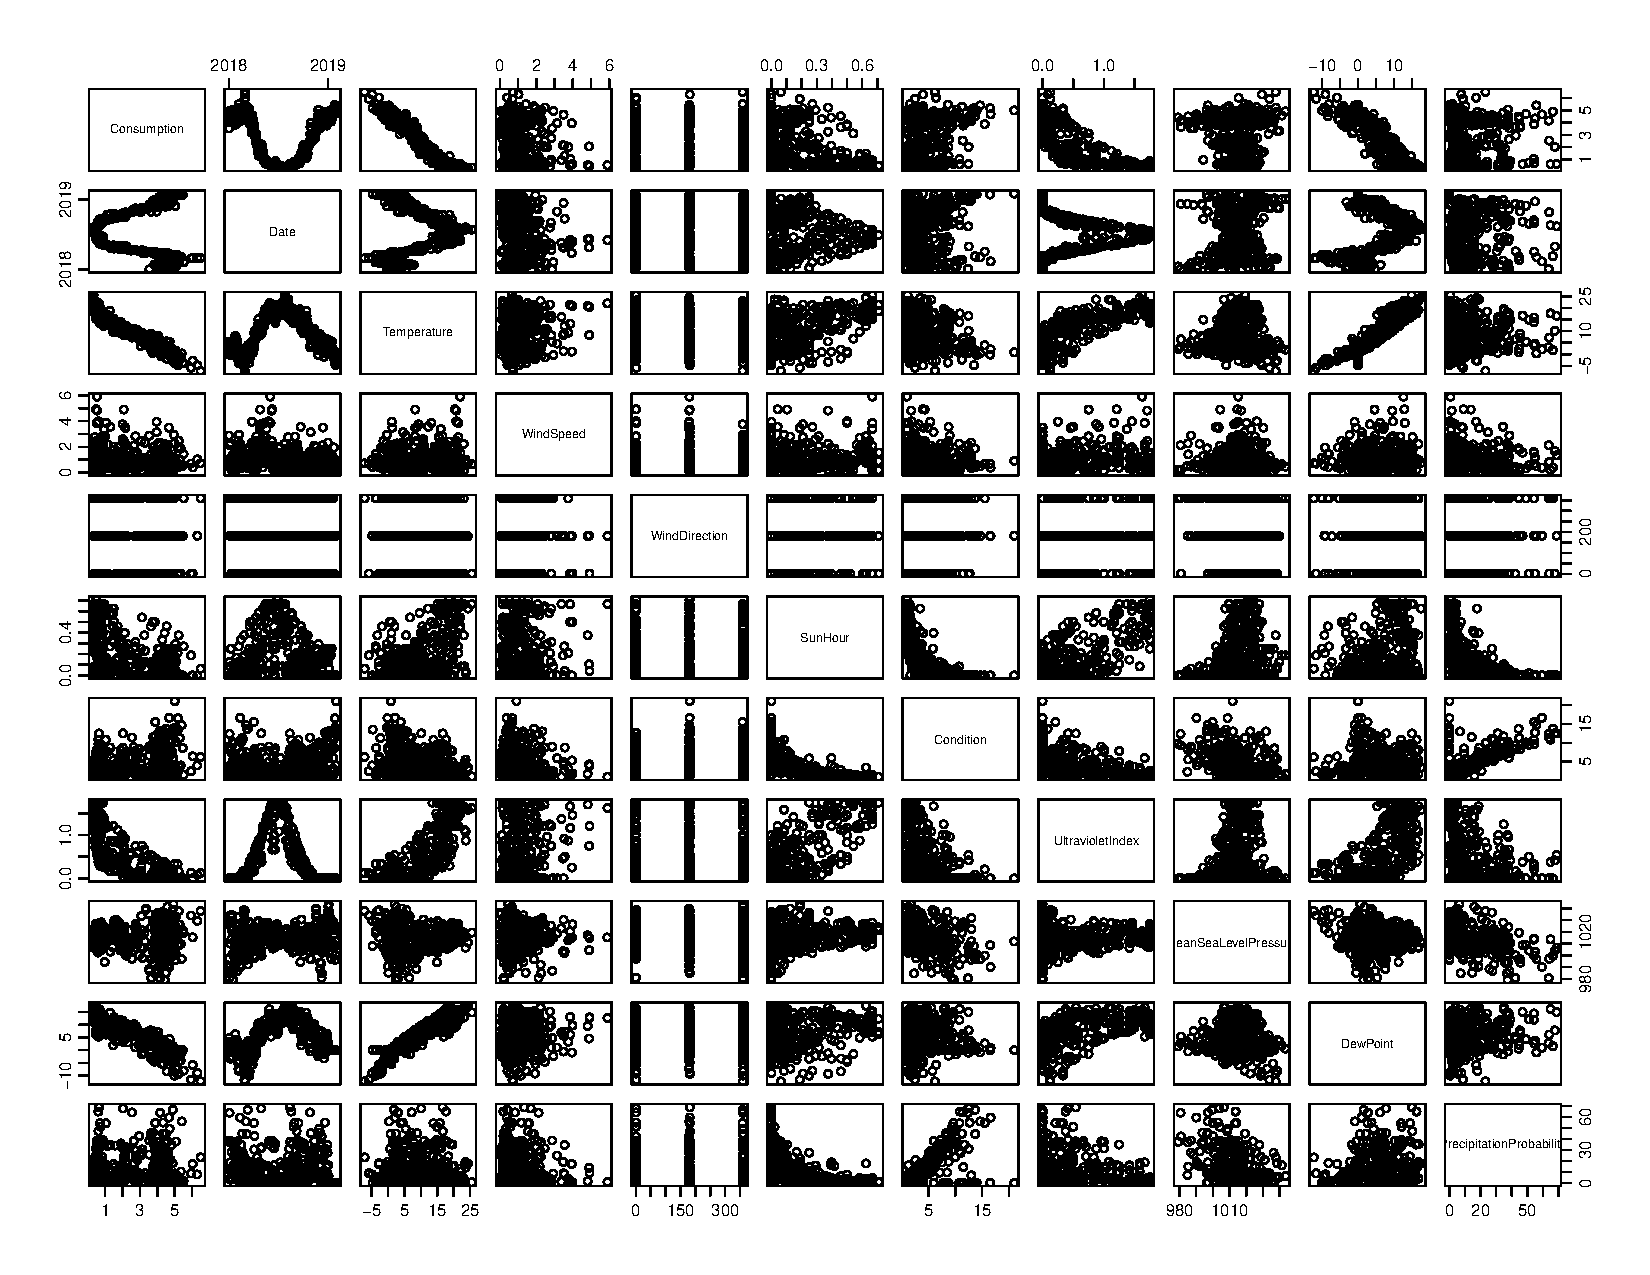
\includegraphics[width=1.3\textwidth, angle = 90]{../../../figures/weather_cons.pdf}
    \caption{Scatterplot showing the average of relevant attributes from weather data}
    \label{fig: weather_cons}
\end{figure}

\begin{figure}
    \centering
    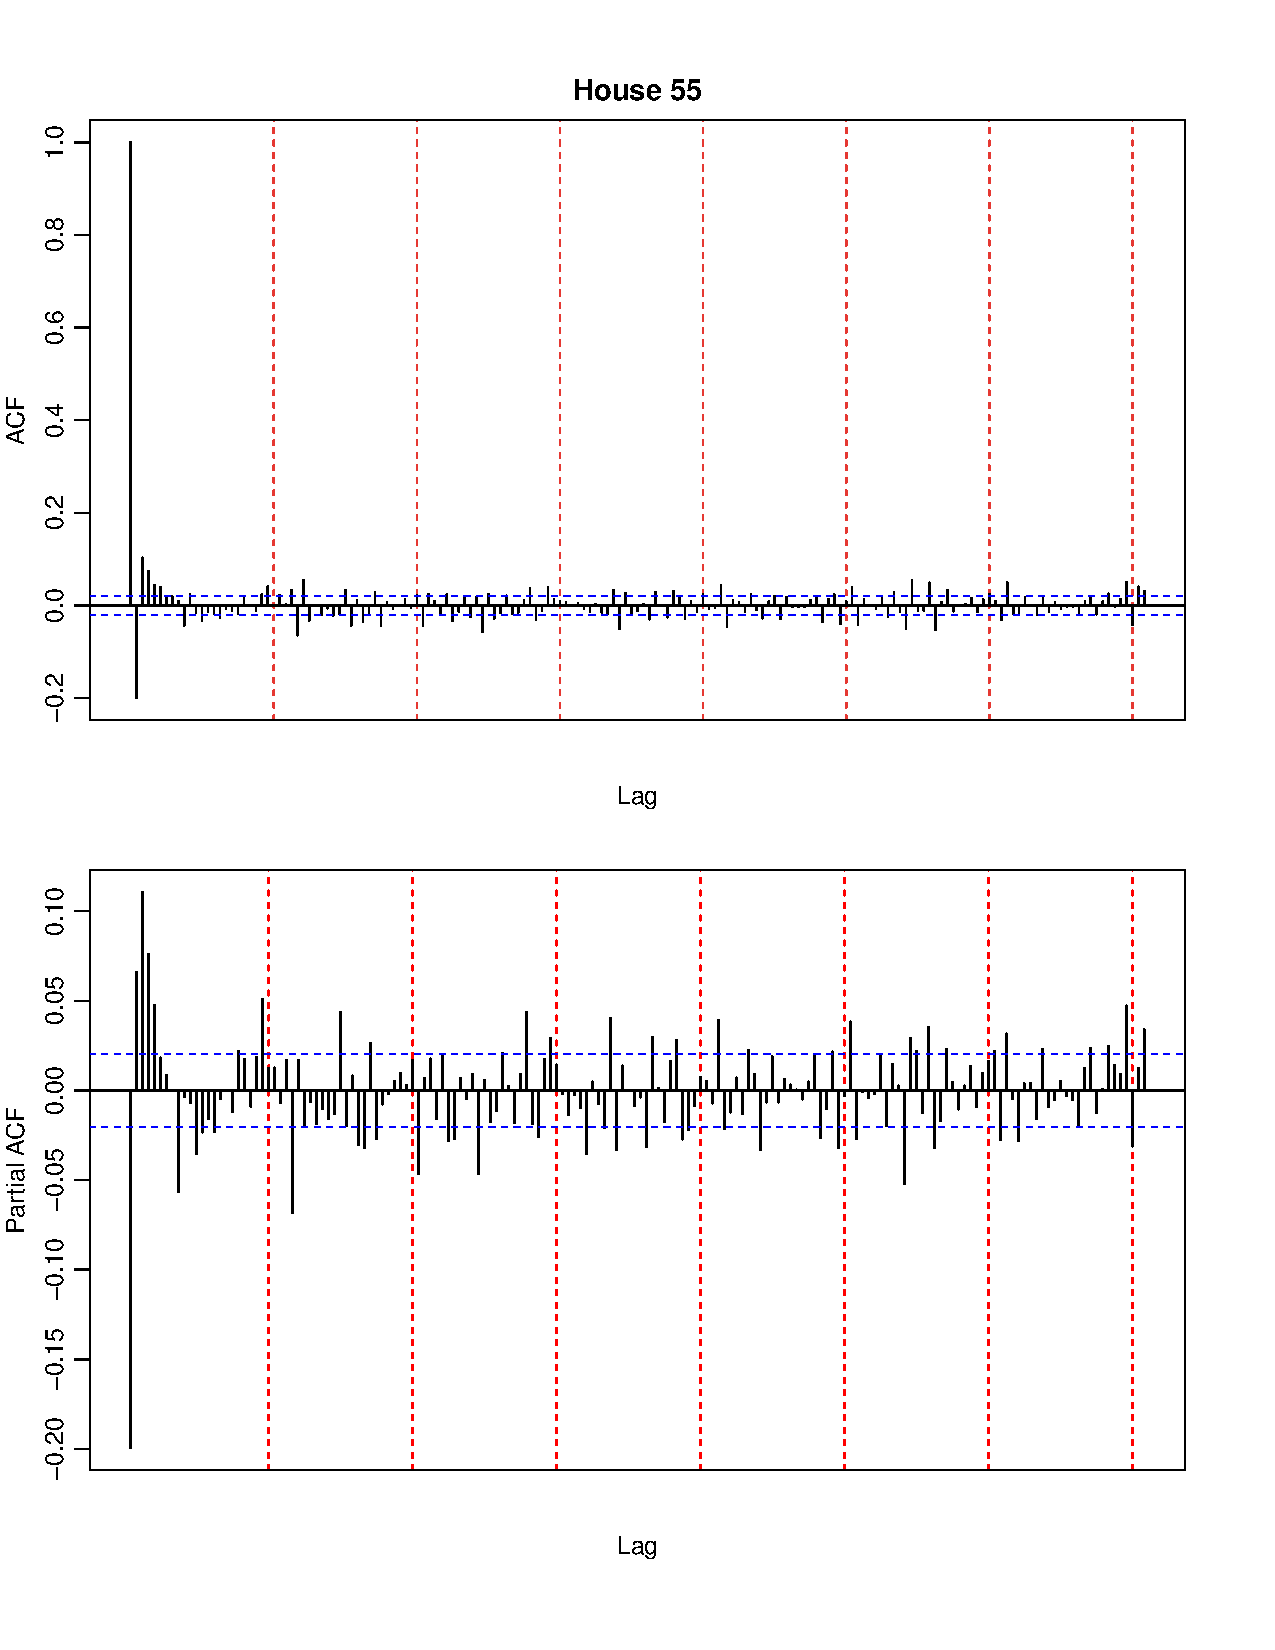
\includegraphics[width=0.8\textwidth]{../../../figures/arimax/ACF_55_long.pdf}
    \caption{The acf and pacf of the second model when applied to house 55}
    \label{fig:Model2_acf_55_long}
\end{figure}    


\begin{figure}
    \centering
    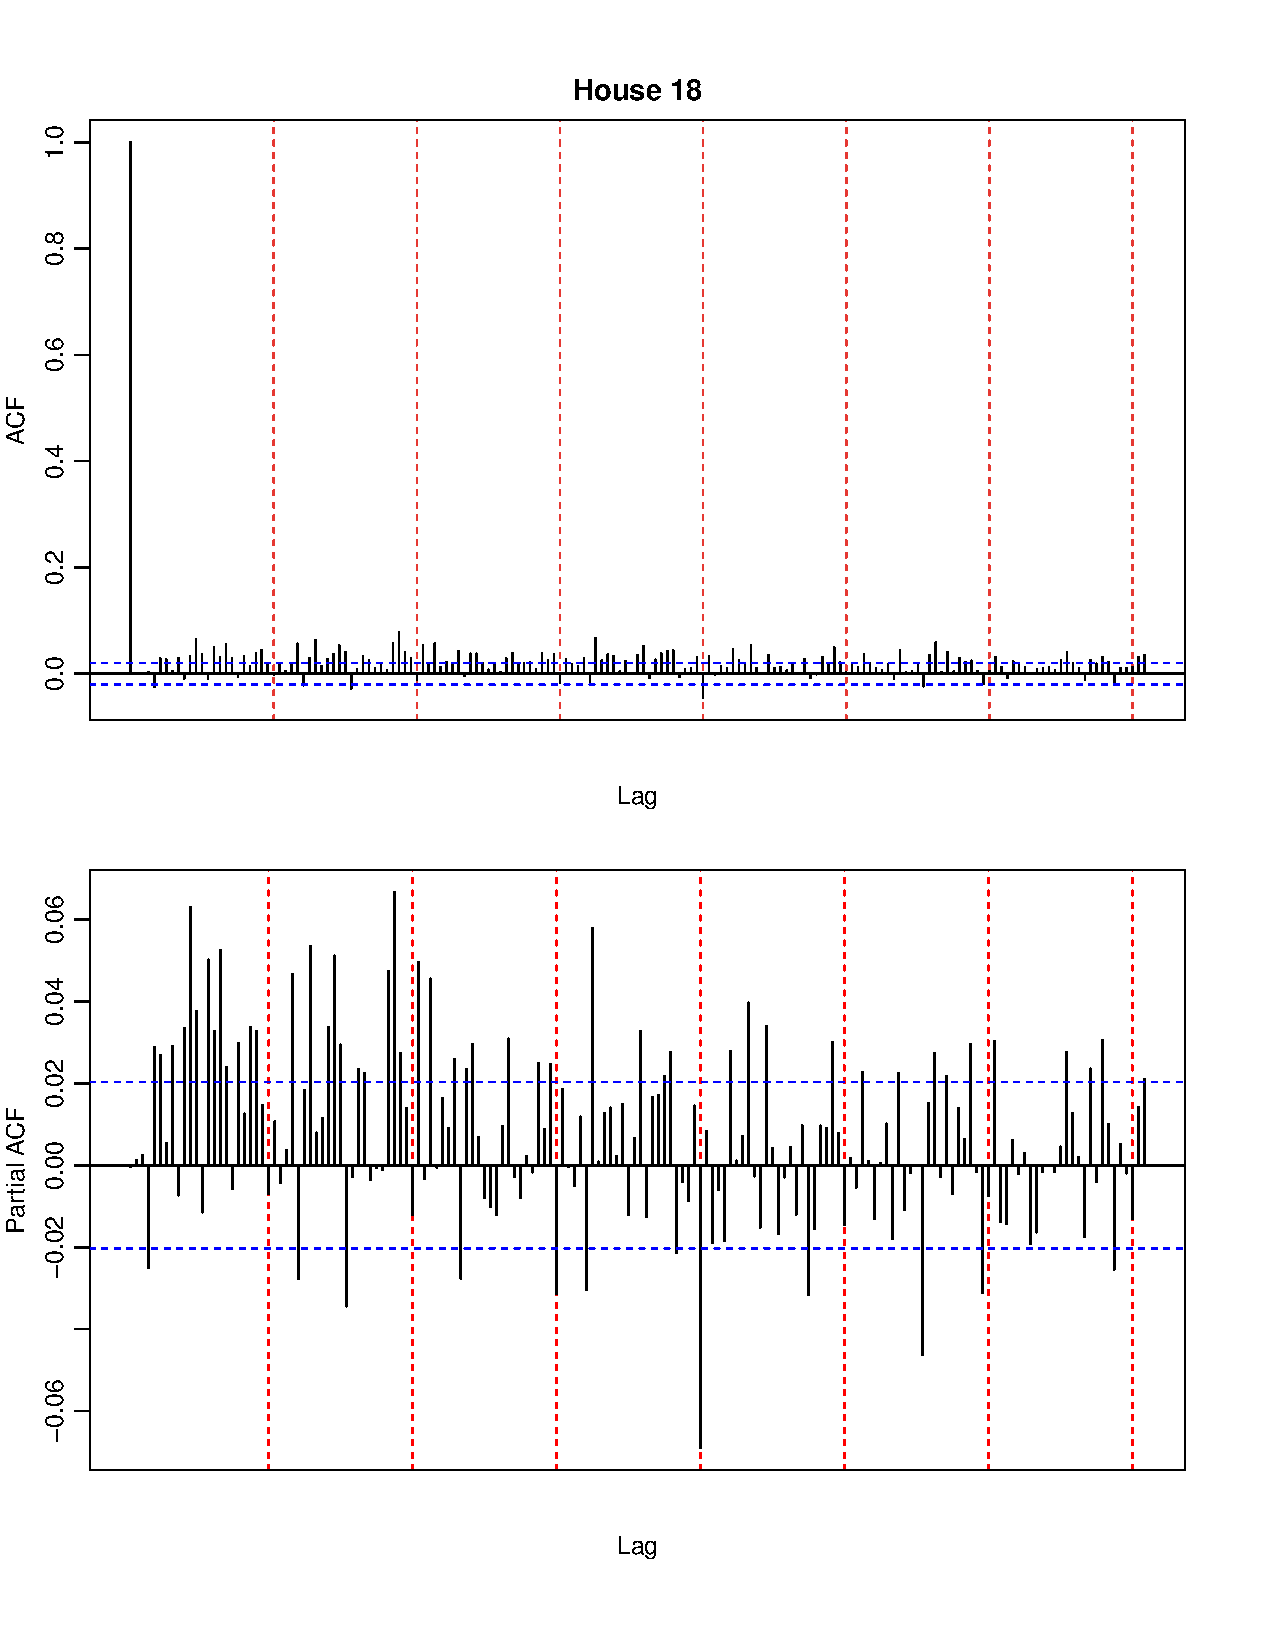
\includegraphics[width=0.8\textwidth]{../../../figures/arimax/ACF_18_long.pdf}
    \caption{The acf and pacf of the second model when applied to house 18}
    \label{fig:Model2_acf_18_long}
\end{figure}    
